\chapter{Implementación del \textit{pipeline} con Dagger}
\label{chap:dagger}

Este capítulo describe la implementación del \textit{pipeline} con Dagger. Se parte de una versión inicial sin la herramienta, y se llega a un ciclo completo, plenamente integrado con esta herramienta. El objetivo es demostrar que Dagger aporta mayor flexibilidad a los desarrolladores para construir \textit{pipelines} de CI y CD, sin depender de tener un entorno de desarrollo ni de una configuración específica para ejecutarlos.

\section{CI}
\label{sec:ci}

Tras realizar una primera aproximación de la aplicación de prueba, el siguiente paso consiste en realizar el ciclo de CI. En este ciclo se realizan los tests de la aplicación, el \textit{linting}, es decir, verificar que el código cumpla ciertos estándares de estilo; y la publicación de imágenes de Docker y de paquetes NPM. Al principio se comenzó a implementar el ciclo completo sin el uso de Dagger. Se utilizó un \texttt{justfile} con los comandos necesarios para realizar tanto los tests como el \textit{linting} de los paquetes de la aplicación, y se crearon dos \textit{scripts}: uno para la publicación de imágenes y otro para la publicación de paquetes NPM. Además, se crea un Dockerfile para poder realizar las pruebas \textit{end-to-end} del \textit{frontend} con Cypress\cite{cypress}.

La desventaja con respecto al Dagger es evidente: \textit{scripts} y comandos que ``funcionan en mi máquina''. Siguiendo esta práctica, sería necesario que todo el equipo de desarrollo utilizara el mismo entorno de desarrollo, y aún así, no se garantizaría el funcionamiento del ciclo de CI, debido a posibles configuraciones que cada desarrollador haya hecho a su sistema que pueda diferir de las configuraciones de los demás. Con este método, los desarrolladores no tienen margen de maniobra en cuanto al sistema que deben utilizar.

Ahora se explica el diseño e implementación con Dagger del mismo ciclo de CI.

Una vez el ciclo de CI sin Dagger se ha realizado al completo, se pasó a traducir los scripts y comandos a un módulo de CI con Dagger, utilizando el SDK de Go.

En la Figura \ref{fig:dagger-ci} se puede comprobar la estructura de este módulo. Se ha optado por implementar un objeto principal \texttt{Ci}, el cual tiene la capacidad de hacer uso de cualquiera de los otros dos objetos customizados, uno específicamente diseñado para gestionar el \textit{frontend} y otro para el \textit{backend}. Este diseño concuerda con la propia estructura y filosofía del \textit{monorepo}: elementos separados que realizan tareas diferentes, pero que se interrelacionan desde un punto central (Lerna para el \textit{monorepo}, y el objeto \texttt{Ci} para el módulo).

\begin{figure}[h]
  \centerline{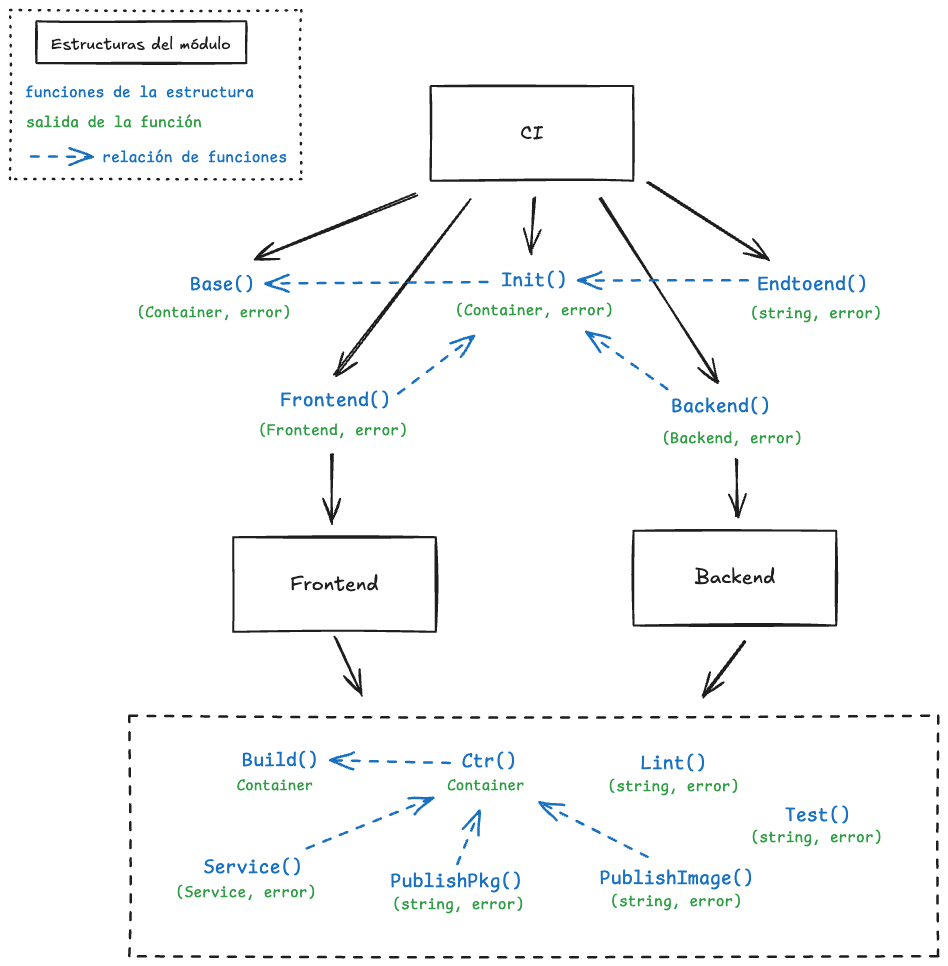
\includegraphics[width=12cm]{figuras/dagger-CI}}
  \caption{Diagrama del diseño del módulo de CI con Dagger. Imagen creada con \href{https://excalidraw.com}{excalidraw.com}}
  \label{fig:dagger-ci}
\end{figure}

Por lo tanto, la idea del diseño del módulo es la misma que la del \textit{monorepo}, tener un elemento principal desde el que hacer uso de cualquiera de los otros tipos customizados\cite{dagger-custom-types}, que se corresponden con los paquetes de la aplicación.

En Dagger se hace uso del ``encadenamiento''. Esto permite llamar a las funciones de los objetos que devuelven las propias funciones. Así, se puede llamar a la función del objeto principal del módulo que devuelve el objeto \texttt{Backend}, y se tendrá acceso a las funciones que están definidas para este paquete.

Para entender cómo funciona, se explicará un ejemplo sencillo con pseudocódigo del propio módulo. En el Listing \ref{lst:chaining-code} se puede ver un ejemplo de dos funciones del módulo de CI (se han escrito comentarios de lo que se hace en el código para reducir su tamaño). La primera función corresponde con el objeto principal del módulo. Este construye la imagen base y posteriormente crea un objeto \texttt{Backend}, el cual devuelve como referencia al final de la función. El hecho de que este objeto sea devuelto por la función, permite acceder a las funciones que este tiene definidas.

Una función definida para \texttt{Backend} es \texttt{Test}, que aparece justo después. En esta se utiliza la imagen base que se ha pasado como parámetro en la construcción del objeto. Se ejecuta dentro del contenedor que define dicha imagen el comando que permite correr los tests del paquete \textit{backend} de la aplicación. Como se puede comprobar, se utiliza Lerna para ejecutar el \textit{script} \texttt{test}, definido en el \texttt{package.json} del paquete correspondiente, indicado mediante el parámetro \textit{scope}.

\begin{longlisting}
  \begin{minted}{go}
// Ci (main.go)

type Ci struct {
	// +required
	SecEnv  *dagger.Secret
	secrets secrets
}

func (m *Ci) Backend(
ctx context.Context,
// +defaultPath="/"
src *dagger.Directory,
) (*Backend, error) {
  base, _ := m.Init(ctx, src)

  // Se obtienen las claves y los valores de los secretos para
  // el *backend*.

  return &Backend{
    Name:    "backend",

    // Imagen base, con todo lo necesario para ejecutar los
    // comandos que se precise.
    Base:    base,

    // Claves y valores de los secretos obtenidos antes.
    Secrets: SecMap{Keys: keys, Values: values},
  }, nil
}

// Backend (backend.go)

func (m *Backend) Test(ctx context.Context) (string, error) {
  return m.Base.
    WithExec([]string{"lerna", "run", "test", "--scope", "@vieites-tfg/zoo-backend"}).
    Stdout(ctx)
}

\end{minted}
\caption{Funciones del módulo de Dagger de CI.}
\label{lst:chaining-code}
\end{longlisting}

La manera en la que se ejecuta a través de un comando la cadena de funciones anterior es como aparece en el Listing \ref{lst:chaining-command}. El comando se realiza en el directorio de trabajo del módulo de CI. Se hace una llamada a Dagger, se pasan los valores requeridos por el módulo, los cuales se indican en la definición del objeto principal; y finalmente se empieza a llamar a las funciones que tiene cada uno de los objetos. A las funciones se las llama en formato ``kebab-case'', aunque en el propio código estén en ``camelCase''. Por lo tanto, primero se realiza la llamada a la función \texttt{backend} y, posteriormente, sabiendo que esta función devuelve un tipo \texttt{Backend}, se llama a la función \texttt{test} que este tiene definida.

\begin{listing}[!ht]
  \begin{minted}{bash}
dagger call --sec-env=file://../../.env backend test
\end{minted}
\caption{Encadenamiento de funciones del módulo de CI.}
\label{lst:chaining-command}
\end{listing}

De esta manera se puede lanzar la función que se prefiera de cualquiera de los paquetes. También, esta estructura y diseño del módulo facilita la escalabilidad de la aplicación, permitiendo añadir fácilmente más paquetes en el caso de ser necesario. Lo único que habría que hacer sería crear un objeto nuevo con funciones para las tareas que se quieran realizar en este, y añadir una función en el objeto principal del módulo que devuelva el nuevo objeto creado para el paquete.

Junto con la ejecución de los tests y del \textit{linter}, se añade también al módulo la posibilidad de levantar por separado cada uno de los paquetes. Esto quiere decir que se permite acceder de manera local a los servicios de los paquetes, la página web por un lado y la API por el otro.

Antes de implementar esa lógica en el módulo de CI, se desarrolla lo necesario para conseguir levantar la aplicación entera de la manera más sencilla posible. En este caso, se utiliza un \texttt{Dockerfile} con varios pasos, en los cuales se construye y se prepara la imagen para la ejecución de cada uno de los paquetes. Esto se consigue con construcciones \textit{multi-stage}, un ejemplo de esto se encuentra en el Listing \ref{lst:dockerfile}.

Con el \texttt{Dockerfile} anterior y con la construcción de un \texttt{docker-compose.yaml}, se consigue levantar la aplicación de manera local. Tras conseguir esto, se traduce de nuevo la lógica al módulo de Dagger. Se crea en cada uno de los objetos del módulo una función \texttt{service}, que permiten levantar los paquetes por separado y acceder a ellos de manera local. Gracias a estas funciones es posible realizar los tests \textit{end-to-end} de la aplicación, donde una única función es capaz de realizar los siguientes pasos:

\begin{itemize}
  \item Tests y \textit{linting} de cada uno de los paquetes.
  \item Levantar los servicios de los paquetes, permitiendo su comunicación de manera interna.
  \item Correr los tests de la aplicación con Cypress.
\end{itemize}

Todo lo anterior integrado en el módulo y ejecutado con una única llamada a una función del objeto principal de la aplicación.

Aquí es donde realmente se ve la potencia de Dagger. Todo se programa en un lenguaje conocido para el desarrollador, con sintaxis que no depende del sistema en el que se está desarrollando y sin la aparición de problemas relacionados con el entorno de ejecución, ya que funciona independientemente del sistema. Esto es gracias a ejecutar todo sobre un \textit{runtime} de OCI, como Docker. Para realizar todo lo anterior sin Dagger, habría que: lanzar los comandos de Lerna de manera local, levantar los servicios con Docker Compose y correr los tests de Cypress con un \texttt{Dockerfile} específico para la causa. Y aún haciendo todo esto, no se tendría la flexibilidad de realizar pruebas y obtener \textit{logs} que se tiene con Dagger. Además, Dagger permite acceder al contenedor en cualquier momento de la ejecución del \textit{pipeline}.

\section{CD}
\label{sec:cd}

El ciclo de CD involucra: la construcción de los recursos de Kubernetes, el encriptado de los secretos y la publicación de todos los manifiestos necesarios en el repositorio de estado.

Para comenzar con este ciclo, se crearon un par de \textit{scripts}, uno que permitía construir las imágenes de Docker y su publicación y otro que facilitaba la publicación de los paquetes NPM. Esto tiene las desventajas ya comentadas, son \textit{scripts} que se ejecutan de manera local y que, por lo tanto, dependen del entorno en el que se ejecutan. En el caso de cambiar de entorno de desarrollo, sería necesario crear nuevos \textit{scripts} o acomodarlos al nuevo entorno. Esto solo trae problemas innecesarios a los desarrolladores, que se tienen que centrar en solucinar estos inconvenientes, externos a la finalidad del desarrollo de la aplicación en sí.

Tras crear los \textit{scripts} anteriores, se pasó a la construcción de las Charts de Helm de la aplicación. Se diseñó la estructura de las Charts y los componentes que iban a tener cada uno de los servicios de la aplicación. Entonces se definieron todos los recursos con Helm y se realizaron pruebas hasta que finalmente todo funcionaba como se esperaba.

La construcción de las Charts era necesario realizarlo tras ser capaz de publicar las imágenes de Docker al Container Registry. Esto es porque Kubernetes utiliza imágenes construidas que obtiene de cualquier registro que se le indique, no se le puede pasar un \textit{Dockerfile} para que construya la imagen.

Todo el proceso de creación de las Charts se ha realizado en local, utilizando comandos de Helm. Una vez comprobada la funcionalidad de esta, se procedió a la separación de responsabilidades: un repositorio para las Charts por un lado (\texttt{helm-repository}), y otro repositorio con los valores que pueblan las Charts por otro lado (\texttt{state}). Esto facilita el desarrollo y mantenimiento de las Charts. Además, se tiene una única fuente de verdad para obtener los valores.

Con los distintos repositorios creados, es necesario utilizar la herramienta \texttt{helmfile} para integrar Charts y valores. El archivo de configuración de esta herramienta se incluye en el repositorio de estado, manteniendo así la norma de tener toda la gestión de valores en un mismo lugar.

Así, ya es posible desplegar la aplicación utilizando Kubernetes. Lo siguiente es hacer uso de Dagger para permitir realizar el despliegue. Se comienza utilizando un método \textit{push} de despliegue. En el propio módulo de Dagger que se creó inicialmente, se utiliza \texttt{helmfile} para desplegar la aplicación en un \textit{cluster} de KinD. No existe ArgoCD, ni varios entornos. Por ahora es sencillo y directo, se crea un \textit{cluster} con un módulo de KinD para Dagger, y se ejecuta el comando de \texttt{helmfile} necesario para desplegar la aplicación.

A continuación se decide emplear el método \textit{pull}, ya comentado, donde existe una herramienta que es la que se encarga de obtener los recursos que se van a desplegar. Esa herramienta es ArgoCD. El módulo de CD de Dagger pasa de desplegar la aplicación a ser el encargado de publicar en la rama \texttt{deploy} del repositorio \texttt{state} los recursos que se van a desplegar en cada entorno. Esto implica

\begin{enumerate}
  \item Realizar el \textit{template} de los recursos con \texttt{helmfile}, es decir, mostrar el renderizado de estos pero sin desplegarlos.
  \item Obtener los secretos y encriptarlos.
  \item Crear los archivos que dice a ArgoCD cómo desencriptar los secretos,
  \item Publicar todo en la rama de despliegue del repositorio de estado.
\end{enumerate}

Tras tener en funcionamiento el módulo, se procede a crear el \textit{workflow} de GitHub, cuyo funcionamiento se explica en la Sección \ref{sec:promotion}. En resumen, se encarga de ejecutar los módulos de CI y CD, ejecutando los tests \textit{end-to-end} previamente a la publicación de las nuevas imágenes de Docker y actualizando el repositorio de estado con la definición de los recursos en el entorno que proceda, utilizando las nuevas imágenes creadas.

De esta manera, se integra todo lo que se ha creado:

\begin{itemize}
  \item Los módulos de Dagger de CI y de CD.
  \item Las Charts de Helm y valores.
  \item Los \textit{clusters} de KinD con los entornos levantados, con ArgoCD instalado en cada uno de ellos.
  \item Un \textit{workflow} de GitHub que enlaza todo lo anterior.
\end{itemize}
